\documentclass[12pt, a4paper]{extarticle}
\usepackage{GOST}

\makeatletter
\renewcommand\@biblabel[1]{#1.}
\makeatother


\graphicspath{{images/}}

\begin{document}
\begin{table}[ht]
	\centering
	\begin{tabular}{|c|p{400pt}|} 
	\hline
		\begin{tabular}[c]{@{}c@{}} 
\includegraphics[scale=0.8]{b_logo} \\\end{tabular} &
		\footnotesize\begin{tabular}[c]{@{}c@{}}\textbf{Министерство~науки~и~высшего~образования~Российской~Федерации}\\\textbf{Федеральное~государственное~бюджетное~образовательное~учреждение}\\\textbf{~высшего~образования}\\\textbf{«Московский~государственный~технический~университет}\\\textbf{имени~Н.Э.~Баумана}\\\textbf{(национальный~исследовательский~университет)»}\\\textbf{(МГТУ~им.~Н.Э.~Баумана)}\\\end{tabular}  \\
	\hline
	\end{tabular}
\end{table}
\noindent\rule{\textwidth}{4pt}
\noindent\rule[14pt]{\textwidth}{1pt}
\hfill 
\noindent
\makebox{ФАКУЛЬТЕТ~}%
\makebox[\textwidth][l]{\underline{~~~~~«Информатика и системы управления»~~~~~~~~~~~~~~~~~~~~~~~~~}}%
\\
\noindent
\makebox{КАФЕДРА~}%
\makebox[\textwidth][l]{\underline{«Программное обеспечение ЭВМ и информационные технологии»}}%

\begin{center}
	\vspace{1.5cm}
	{\bf\huge Расчетно-пояснительная записка\par}
	{\bf\Large к курсовой работе\par}
	\vspace{0cm}
\end{center}


\noindent
\makebox{\large{\bf Тема:}~~~}
\makebox[\textwidth][l]{\large\underline{~Разработка протокола с дедупликацией~~~~~~~~~~~~~}}\\

\noindent
\makebox{\large{\bf Дисциплина:}~~~}
\makebox[\textwidth][l]{\large\underline{~Компьютерные сети~~~~~~~~~~~~~~~~~~~~}}\\

\vspace{1cm}
\noindent
\begin{tabular}{l c c c c c}
    Студент      & ~ИУ7-75Б~       & \hspace{2.5cm} & \hspace{3cm}               & &  П.К Хетагуров \\\cline{2-2}\cline{4-4} \cline{6-6} 
    \hspace{3cm} & {\footnotesize(Группа)} &                & {\footnotesize(Подпись, дата)} & & {\footnotesize(И.О. Фамилия)}
\end{tabular}

\vspace{0.5cm}

\noindent
\begin{tabular}{l c c c c}
    Руководитель проекта & \hspace{3.3cm}   & \hspace{3.5cm}              & & Н.О. Рогозин \\\cline{3-3} \cline{5-5} 
    \hspace{2.9cm}  &              & {\footnotesize(Подпись, дата)} & & {\footnotesize(И.О. Фамилия)}
\end{tabular}

\begin{center}	
	\vfill
	\large \textit {Москва, 2021}
\end{center}

\thispagestyle {empty}
\pagebreak
\section{Задание}

Для общей сети был выделен частный адрес 192.168.x.0/24

Задачи:
\begin{enumerate}
\item Разделить сеть на 5 подсетей
	 \begin{enumerate}
	\item Подсети 1 и 5 должны поддерживать до 10 +  x устройств
	\item Подсети 2 и 4 должны поддерживать до 5 устройств
	\item Подсеть 3 должна поддерживать 2 устройства
	\end{enumerate}

	Где x - Ваш номер по списку в ЭУ

	Использовать не более трех подсетей с возможностью размещения x + 10 хостов

\item Настроить  DHCP-сервера для выдачи адресов
 	\begin{enumerate}
	\item Для подсети 1 настроить отдельный DHCP сервер	
	\item Для подсети 2 настроить в качестве DHCP-сервера маршрутизатор 1
	\item Для подсетей 4 и 5 настроить в качестве DHCP-сервера маршрутизатор 2
	\end{enumerate}
\end{enumerate}

\section{Результаты}
Подсети 1 и 5 в моем варианте должны поддерживать 14 + 10 = 24 хоста. \\
Сначала были выделены подсети 1 и 5, затем 2 и 4, последней была выделена подсеть 3. Выделение происходило в порядке убывания числа хостов. Не учитывались адрес сети и широковещательный домен при определении кол-ва хостов.
\begin{table}[H]
	\centering
	\caption{Адреса подсетей}
	\begin{tabular}{| c |  c | c | c |}
	\hline
	Номер подсети & Адрес сети & Маска подсети & Кол-во хостов \\ \hline
	1 & 192.168.14.0 & 255.255.255.224 & 30 \\ \hline
	5 & 192.168.14.32 & 255.255.255.224  & 30 \\ \hline
	2 & 192.168.14.64 & 255.255.255.248 & 6 \\ \hline
	4 & 192.168.14.72 & 255.255.255.248 & 6 \\ \hline
	3 & 192.168.14.60 & 255.255.255.252 & 2 \\
	\hline
	\end{tabular}
\end{table}
Шлюзам по умолчанию выдавался первый адрес из диапазона.

\begin{figure}[H]
	\centering
	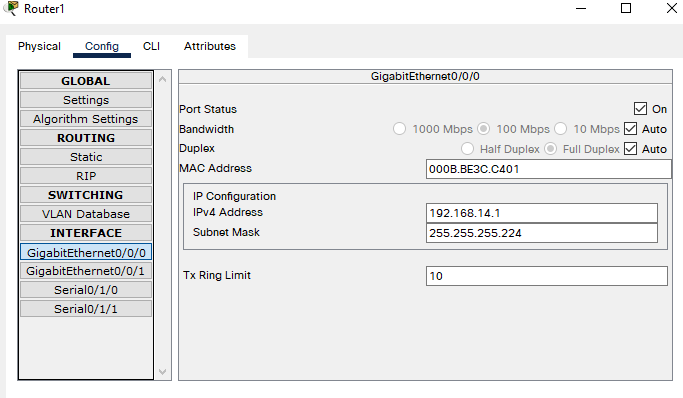
\includegraphics[scale=0.9]{images/router1.png}
	\caption{Настройка интерфейса для подсети 1 на роутере 1}
\end{figure}

Настройка DHCP.
\begin{figure}[H]
	\centering
	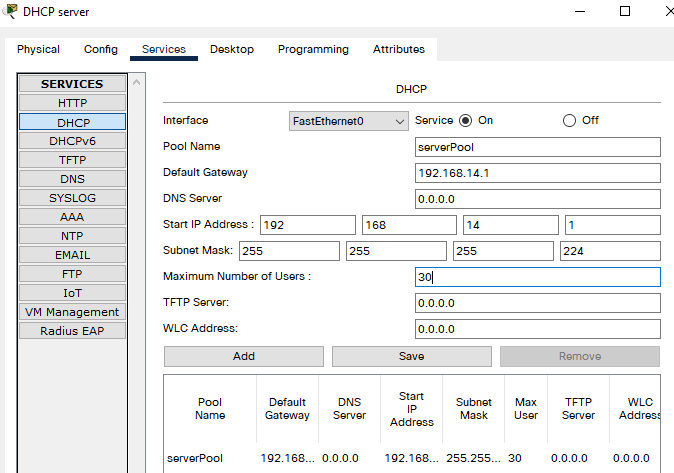
\includegraphics[scale=0.9]{images/dhcp.png}
	\caption{Настройка DHCP сервера}
\end{figure}

\begin{figure}[H]
	\centering
	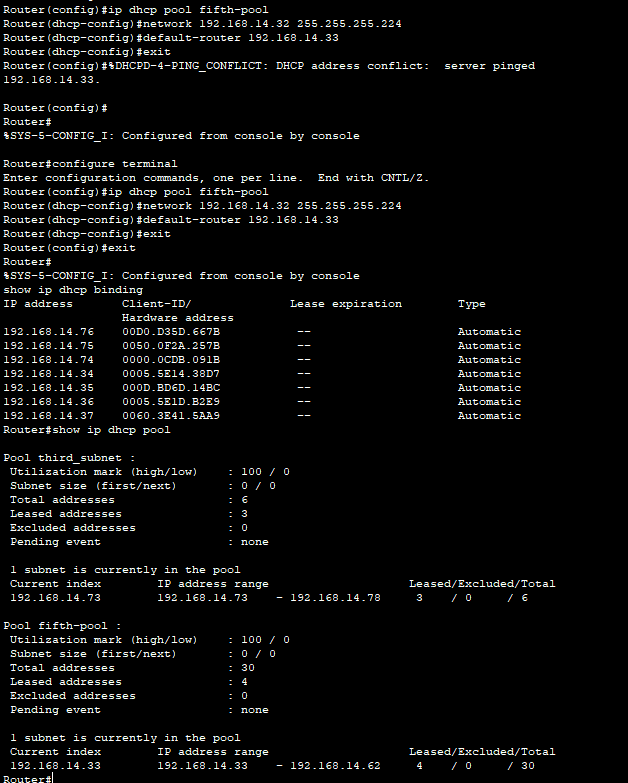
\includegraphics[scale=0.9]{images/dhcp-set.png}
	\caption{Настройка DHCP на роутере 2 для подсетей 4 и 5}
\end{figure}

Для связи подсетей за роутером 1 и подсетей за роутером 2 были добавлены статические пути на роутере 1 и 2.
\begin{figure}[H]
	\centering
	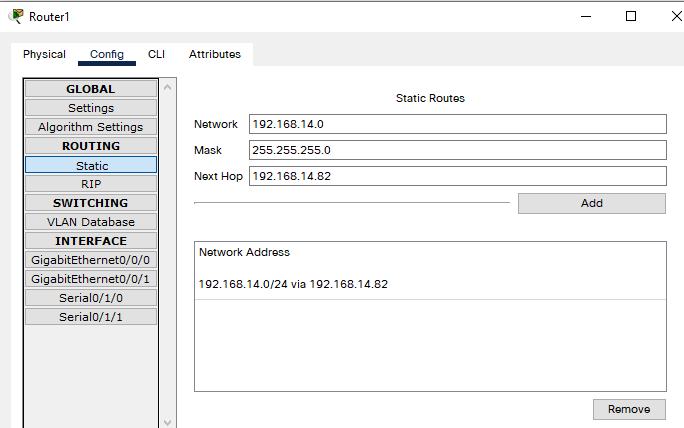
\includegraphics[scale=0.9]{images/static.png}
	\caption{Статический путь на роутере 1}
\end{figure}

В результате все подсети пингуются.
\begin{figure}[H]
	\centering
	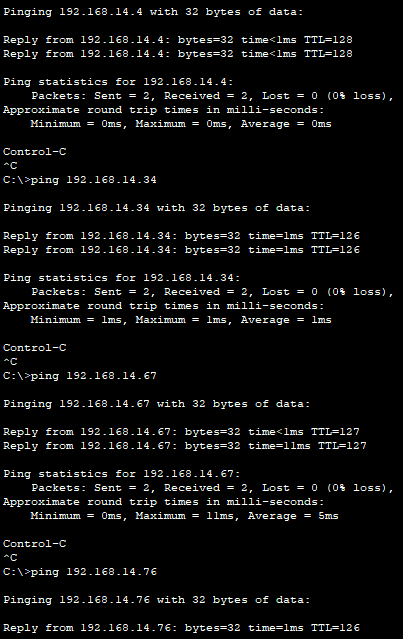
\includegraphics[scale=0.9]{images/ping.png}
	\caption{Пинг из подсети 1}
\end{figure}
\end{document}




